\documentclass[a4paper,12pt]{article}
\usepackage{graphicx} 
\usepackage{hyperref}
\usepackage{float}
\usepackage{amsmath}
\usepackage{amssymb}  % For \mathbb
\usepackage{enumitem}


% \begin{figure}[H]
%     \centering
%     \includegraphics[width=0.7\textwidth]{filename.png}
%     \caption{Your figure caption here.}
%     \label{fig:yourlabel}
% \end{figure}

\begin{document}

\title{Assignment 4 - Data Science \\
Theoretical Questions}
\author{Mohammad Hossein Basouli}
\date{\today}
\maketitle

\section*{Question 1}

\begin{enumerate}[label=(\alph*)]
    \item 
    \begin{enumerate}[label=\arabic*.]
        \item \textbf{Sensors \& Preprocessing}: Use sensors to receive signals, and apply preprocessing to improve data quality.
        \item \textbf{Feature Extraction}: Extract useful features from raw feature vectors. 
        \item \textbf{Learning Algorithm}: The utilized algorithm to learn the pattern from the data.
        \item \textbf{Teacher}: Tells the class that each data point belongs to.
    \end{enumerate}
    \item 
    \begin{enumerate}[label=\arabic*.]
        \item \textbf{Teacher}: The teacher provides information about the hidden state of the data points, to the learning algorithm.
        \item \textbf{Learning Algorithm}: Takes the data points (which have, \textbf{Preprocessing} \& \textbf{Feature Extraction} applied on them already) along with the information provided by the teacher by the hidden state of the data points, to learn the pattern that underlies in the dataset.
    \end{enumerate}
    \item In the \textbf{Training Mode}, we first apply \textbf{Preprocessing} \& \textbf{Feature Extraction/Selection} on the training samples, and then feed them to the \textbf{Learning Algorithm}, to try to learn the pattern that underlies in the dataset. But in \textbf{Classification Mode}, we will apply the utilized \textbf{Preprocessing} \& \textbf{Feature Extraction/Selection} in the \textbf{Training Mode}, to the test samples and then feed it to the \textbf{Classification} model that has been obtained from the \textbf{Learning Algorithm}, in order to classify each test sample.
\end{enumerate}

\section*{Question 2}
\begin{enumerate}[label=(\alph*)]
    \item In \textbf{Classification}, we try to predict the class that the sample belongs to, which is a discerete number. But in \textbf{Regression}, we predict a continious number \textit{y}, which we have learnt it's relationship with a set of feature vectors \textit{X} before.
    \item I have already determined the type of output for each one. Now we get to showing one application for each of them: 
    \begin{itemize}
        \item \textbf{Classification}: Optical character recognition
        \item \textbf{Regression}: Prediction of the amount of sales for a icecream shop in the next month.
    \end{itemize} 
\end{enumerate}

\section*{Question 3}
\begin{enumerate}[label=(\alph*)]
    \item It represents a vector of observations (measurements).
    \item It determines the class that the given sample belongs to, and could be used in order to learn the pattern between the feature vectors and the hidden states of some given samples. 
\end{enumerate}

\section*{Question 4}
\begin{enumerate}[label=(\alph*)]
    \item It stores the feature vectors along with hidden states for all of the training samples, and then given a new sample $X$, it will lookup the stored training sample $X_i$ such that $X_i = X$ and then it will output the hidden state of the sample $X_i$ as the predicted hidden state for $X$.
    \item Some images might not be recognized.
\end{enumerate}

\section*{Question 5}
\begin{enumerate}[label=(\alph*)]
    \item The area/region that all of the points in it, belong to the sample class, form a \textbf{Decision Region}.
    \item The boundary between different \textbf{Deicision Regions} is called \textbf{Decision Boundary}. Illustration is given in Figure~\ref{fig:fig_1}
    \begin{figure}[H]
        \centering
        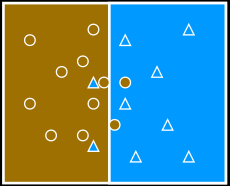
\includegraphics[width=0.7\textwidth]{../images/decision_boundary.png}
        \caption{Illustration of The Decision Boundary. The white line on the middle, that separates the two classes, illustrates the decision boundary in this problem.}
        \label{fig:fig_1}
    \end{figure}
\end{enumerate}

\section*{Question 6}
\textit{note: I have used the GPT to write out formula for \textbf{Bayesian Theorem} and explain the terms in it, but i'm fully aware of what is going on and what's the logic behind all these.}
\begin{enumerate}[label=(\alph*)]
    \item Bayes' Theorem in the Context of Classification:
    \[
    P(C_k \mid \mathbf{x}) = \frac{P(\mathbf{x} \mid C_k) \cdot P(C_k)}{P(\mathbf{x})}
    \]

    Where:
    \begin{itemize}
        \item $C_k$ is the $k$-th class.
        \item $\mathbf{x}$ is the feature vector (observation).
        \item $P(C_k \mid \mathbf{x})$ is the posterior probability of class $C_k$ given observation $\mathbf{x}$.
        \item $P(\mathbf{x} \mid C_k)$ is the likelihood of observing $\mathbf{x}$ given class $C_k$.
        \item $P(C_k)$ is the prior probability of class $C_k$.
        \item $P(\mathbf{x})$ is the evidence or marginal likelihood.
    \end{itemize}

    \item Decision Rule for Classification:
    Assign observation $\mathbf{x}$ to the class with the highest posterior probability:
    \[
    \hat{C} = \arg\max_{C_k} P(C_k \mid \mathbf{x})
    \]

    Using Bayes' theorem, this becomes:

    \[
    \hat{C} = \arg\max_{C_k} \left[ P(\mathbf{x} \mid C_k) \cdot P(C_k) \right]
    \]

    Since $P(\mathbf{x})$ is constant for all classes, it can be omitted in the maximization.

    \item Explanation of Terms in Bayes' Theorem:
    \begin{itemize}
        \item \textbf{Prior} ($P(C_k)$): The prior probability represents our initial belief about the probability of class $C_k$ before observing any data. It reflects how common or likely a class is in general.

        \item \textbf{Likelihood} ($P(\mathbf{x} \mid C_k)$): The likelihood is the probability of observing the data $\mathbf{x}$ given that the class is $C_k$. It models how probable the observed features are under the assumption that the data comes from class $C_k$.

        \item \textbf{Posterior} ($P(C_k \mid \mathbf{x})$): The posterior probability is the updated probability of class $C_k$ after observing the data $\mathbf{x}$. It combines the prior and the likelihood to give a more informed estimate.

        \item \textbf{Evidence} ($P(\mathbf{x})$): The evidence (also called the marginal likelihood) is the total probability of observing the data $\mathbf{x}$ across all possible classes. It serves as a normalization constant to ensure the posterior probabilities sum to one:
        \[
        P(\mathbf{x}) = \sum_{j} P(\mathbf{x} \mid C_j) \cdot P(C_j)
        \]
    \end{itemize}
\end{enumerate}

\section*{Question 7}
\begin{enumerate}[label=(\alph*)]
    \item Because when we want to predict posterior probability $P(C_k|x)$ for class $k$, we need to calculate $likelihood = P(x|C_k)$ for each class $k$, and that requires us to be able to estimate PDF.
    \item Parametric estimation is when the density function is known but it's parameters are unknown. Non-parametric is when both are unknown. Examples for each:
    \begin{itemize}
        \item \textbf{Parametric}: Maximum Likelihood Estimation. 
        \item \textbf{Non-parametric}: Parzen Windows, K-NN, etc.
    \end{itemize}
\end{enumerate}

\section*{Question 8}
\begin{enumerate}[label=(\alph*)]
    \item Each of the colors, grey and white, form a separate decision region, and the boundary between these two regions is decision boundary. 
    \item There will be multiple cases:
    \begin{itemize}
        \item \textbf{Overfitted Model}: If the utilized model is overfitted on the training data, the decision regions will be smalled and the decision boundary will have a jagged, irregular pattern. 
        \item \textbf{Moderate/Underfitted Model}: If the model is Moderate or Underfitted on the training data, the decision boundaries would be smoother.
    \end{itemize}
\end{enumerate}

\section*{Question 9}
\begin{enumerate}[label=(\alph*)]
    \item It finds the first nearest neighbor of a given test sample, and then it will the test sample, to the class of that neighbor.
    \item It doesn't require any training, it just memorizes the training samples, and then it will find the most similar training sample, to a given unseen test sample, and assign the class of that similar training sample to it.
    \item The choice of metric could significantly affect the classifier's accuracy. e.g. if we take \textbf{Euclidian Distance} between the two signals given in the Figure~\ref{fig:fig_2}, we will possibly get a really high number, meaning that these two signals are very disimilar, but if fact these two signals might convey a similar behavior in our point of view; e.g. we might just care about whether these two signals go up and down together or not. Thus using a distance metric such as \textbf{Correlation} would be better for this case.
    \begin{figure}[H]
        \centering
        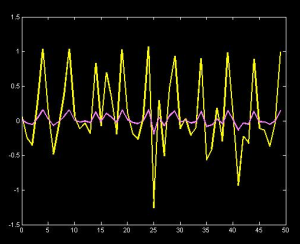
\includegraphics[width=0.7\textwidth]{../images/metric_for_classifier.png}
        \caption{Two signals that their \textbf{Euclidian Distance} is so high but their \textbf{Correlation} about 1.}
        \label{fig:fig_2}
    \end{figure}
\end{enumerate}

\section*{Question 10}
\textit{note: I have used the GPT to write out the steps performed in \textbf{Parzen Windows} method as well as it's formula, but i'm fully aware of why it works like this or what's the logic behind the fomrula for estimating the PDF.}
\begin{enumerate}[label=(\alph*)]
    \item Describe the \textbf{Parzen Window} method for estimating a PDF:
    \textbf{How it works}:
    \begin{itemize}
    \item Place a \textit{kernel/window function} (e.g., mostly \textbf{Gaussian} ) centered at each data point.
    \item Each kernel has a fixed \textbf{bandwidth parameter $h$}, which controls its spread.
    \item The estimated PDF at any point $x$ is the sum of all kernel values at $x$, normalized by the number of data points.
    \end{itemize}

    Mathematically:
    \[
    \hat{p}(x) = \frac{1}{n h^d} \sum_{i=1}^n K\left(\frac{x - x_i}{h}\right)
    \]
    where:
    \begin{itemize}
    \item $K$ is the kernel function,
    \item $h$ is the window width (bandwidth),
    \item $d$ is the number of dimensions,
    \item $n$ is the number of samples.
    \end{itemize}

    \item How does k-NN PDF estimation differ from Parzen?
    In \textbf{k-NN PDF estimation}, the volume around a point is \textit{adjusted}, rather than fixing the window size.
    \textbf{Key differences}:
    \begin{itemize}
    \item \textbf{Parzen:} Fixed window size $h$, variable number of points inside.
    \item \textbf{k-NN:} Fixed number of neighbors $k$, variable volume enclosing those neighbors.
    \end{itemize}

    Mathematically:
    \[
    \hat{p}(x) = \frac{k}{n V_k(x)}
    \]
    where:
    \begin{itemize}
    \item $V_k(x)$ is the volume containing the $k$ nearest neighbors of $x$,
    \item $n$ is the number of samples.
    \end{itemize}

    \item What are the challenges in selecting parameters $h$ or $k$?
    \begin{itemize}
        \item If we choose a very large $h$ we might lose the \textbf{Local Density Estimation} property, which essentially says that the points closer to each center should have a much higher impact than those which are far away from it. (or maybe we should neglect the impact of those which are far apart from the center.)
        \item If we choose a very small $h$ we might lose a significant amount of information, provided by the points which are even a bit relatively further away from the center.
        \item Chosing a very large $k$ is leads to some issue similar to chosing a very large $h$, which has been explain already.
        \item Chosing a very small $k$ is leads to some issue similar to chosing a very small $h$, which has been explain already.
    \end{itemize}
\end{enumerate}

\section*{Question 11}
\begin{enumerate}[label=(\alph*)]
    \item Is a function that provides us with a way to make a distinction between the samples of multiple classes.
    \item Discriminant Function for Multivariate Gaussian Classes:
    
    Given a multivariate normal distribution for class \( \omega_i \) with mean vector \( \boldsymbol{\mu}_i \) and covariance matrix \( \boldsymbol{\Sigma}_i \), the class-conditional density is:

    \[
    p(\boldsymbol{x} \mid \omega_i) = \frac{1}{(2\pi)^{d/2} |\boldsymbol{\Sigma}_i|^{1/2}} \exp\left( -\frac{1}{2} (\boldsymbol{x} - \boldsymbol{\mu}_i)^T \boldsymbol{\Sigma}_i^{-1} (\boldsymbol{x} - \boldsymbol{\mu}_i) \right)
    \]

    The discriminant function \( g_i(\boldsymbol{x}) \) used in Bayesian classification is:

    \[
    g_i(\boldsymbol{x}) = -\frac{1}{2} \ln |\boldsymbol{\Sigma}_i|
    - \frac{1}{2} (\boldsymbol{x} - \boldsymbol{\mu}_i)^T \boldsymbol{\Sigma}_i^{-1} (\boldsymbol{x} - \boldsymbol{\mu}_i)
    + \ln P(\omega_i)
    \]

    \noindent
    Where:
    \begin{itemize}
        \item \( \boldsymbol{x} \in \mathbb{R}^d \) is the feature vector
        \item \( \boldsymbol{\mu}_i \) is the mean vector of class \( \omega_i \)
        \item \( \boldsymbol{\Sigma}_i \) is the covariance matrix of class \( \omega_i \)
        \item \( |\boldsymbol{\Sigma}_i| \) is the determinant of the covariance matrix
        \item \( P(\omega_i) \) is the prior probability of class \( \omega_i \)
    \end{itemize}
\end{enumerate}

\section*{Question 12}
\begin{enumerate}[label=(\alph*)]
    \item Explaining how the EM algorithm is used to estimate parameters in a Gaussian mixture:
    The \textbf{Expectation-Maximization (EM)} algorithm is used to estimate parameters of a \textbf{Gaussian Mixture Model (GMM)} --- a probabilistic model that represents the data as a mixture of several Gaussian distributions.

    Let the parameters of the model be:
    \[
    \theta = \left\{ \pi_k, \mu_k, \Sigma_k \right\} \quad \text{for } k = 1, 2, \dots, K
    \]
    where:
    \begin{itemize}
        \item \( \pi_k \) is the mixing coefficient of component \( k \),
        \item \( \mu_k \) is the mean of component \( k \),
        \item \( \Sigma_k \) is the covariance matrix of component \( k \),
        \item \( \mathcal{N}(x_i \mid \mu_k, \Sigma_k) \) is the Gaussian density function.
    \end{itemize}

    \textbf{EM Algorithm Steps:}
    \begin{enumerate}
        \item \textbf{Initialization:} Choose initial values for \( \pi_k, \mu_k, \Sigma_k \).

        \item \textbf{E-step (Expectation):} Compute the \textit{responsibilities}:
        \[
        \gamma_{ik} = \frac{ \pi_k \, \mathcal{N}(x_i \mid \mu_k, \Sigma_k) }{ \sum_{j=1}^{K} \pi_j \, \mathcal{N}(x_i \mid \mu_j, \Sigma_j) }
        \]

        \item \textbf{M-step (Maximization):} Update the parameters:
        \[
        \pi_k^{\text{new}} = \frac{1}{n} \sum_{i=1}^{n} \gamma_{ik}
        \]
        \[
        \mu_k^{\text{new}} = \frac{ \sum_{i=1}^{n} \gamma_{ik} x_i }{ \sum_{i=1}^{n} \gamma_{ik} }
        \]
        \[
        \Sigma_k^{\text{new}} = \frac{ \sum_{i=1}^{n} \gamma_{ik} (x_i - \mu_k^{\text{new}})(x_i - \mu_k^{\text{new}})^T }{ \sum_{i=1}^{n} \gamma_{ik} }
        \]

        \item \textbf{Repeat} E-step and M-step until convergence.
    \end{enumerate}

    \item Why might ensemble methods outperform a single classifier?
    \begin{itemize}
        \item \textbf{Robustness:} Ensembles are less sensitive to noise and outliers.
        \item \textbf{Improved Accuracy:} By leveraging diversity among base learners, ensembles often achieve higher predictive accuracy.
    \end{itemize}
\end{enumerate}


\end{document}